%\iffalse
\documentclass[12pt]{article}
\usepackage{graphicx}
%\documentclass[journal,12pt,twocolumn]{IEEEtran}
\usepackage[none]{hyphenat}
\usepackage{graphicx}
\usepackage{listings}
\usepackage[english]{babel}
\usepackage{graphicx}
\usepackage{caption} 
\usepackage{hyperref}
\usepackage{booktabs}
\usepackage{array}
\usepackage{amsmath}   % for having text in math mode
\usepackage{listings}
\lstset{
  frame=single,
  breaklines=true
}
  
%Following 2 lines were added to remove the blank page at the beginning
\usepackage{atbegshi}% http://ctan.org/pkg/atbegshi
\AtBeginDocument{\AtBeginShipoutNext{\AtBeginShipoutDiscard}}
%


%New macro definitions
\newcommand{\mydet}[1]{\ensuremath{\begin{vmatrix}#1\end{vmatrix}}}
\providecommand{\brak}[1]{\ensuremath{\left(#1\right)}}
\providecommand{\norm}[1]{\left\lVert#1\right\rVert}
\newcommand{\solution}{\noindent \textbf{Solution: }}
\newcommand{\myvec}[1]{\ensuremath{\begin{pmatrix}#1\end{pmatrix}}}
\let\vec\mathbf

\begin{document}

\begin{center}
\title{\textbf{Properties of Quadrilaterals}}
\date{\vspace{-5ex}} %Not to print date automatically
\maketitle
\end{center}

\setcounter{page}{1}



\section{10$^{th}$ Maths - Chapter 7}

This is Problem-8 from Exercise 7.4

\begin{enumerate}
\item ABCD is a rectangle formed by the points $\vec{A}(–1, –1), \vec{B}(– 1, 4), \vec{ C}(5, 4) \text{ and } \vec{D}(5, – 1)$. $\vec{P,Q,R} \text{ and } \vec{S}$ are the mid-points of $\vec{AB, BC, CD} \text{ and } \vec{DA}$ respectively. Is the quadrilateral
PQRS a square? a rectangle? or a rhombus? Justify your answer. \\
\solution 
Refer figure \ref{fig:Fig3}
\begin{align}
  \label{eq:det2f}
  \vec{P} &= \frac{1}{2}\brak{\vec{A}+\vec{B}} =   \frac{1}{2}\brak{\myvec{
  -1 \\
  -1 \\
 } + \myvec{
  -1 \\
  4 \\
 } 
 } = \myvec{
 -1 \\
 \frac{3}{2} \\
 }   \\
 \vec{Q} &= \frac{1}{2}\brak{\vec{B}+\vec{C}} =   \frac{1}{2}\brak{\myvec{
  -1 \\
  4 \\
 } + \myvec{
  5 \\
  4 \\
 } 
 } = \myvec{
 2 \\
 4 \\
 }   \\
 \vec{R} &= \frac{1}{2}\brak{\vec{C}+\vec{D}} =   \frac{1}{2}\brak{\myvec{
  5 \\
  4 \\
 } + \myvec{
  5 \\
  -1\\
 } 
 } = \myvec{
 5 \\
 \frac{3}{2} \\
 }   \\
 \vec{S} &= \frac{1}{2}\brak{\vec{D}+\vec{A}} =   \frac{1}{2}\brak{\myvec{
  5 \\
  -1 \\
 } + \myvec{
  -1 \\
  -1\\
 } 
 } = \myvec{
 2\\
 -1 \\
 }   \\
\end{align}

\begin{figure}[!h]
	\begin{center}
		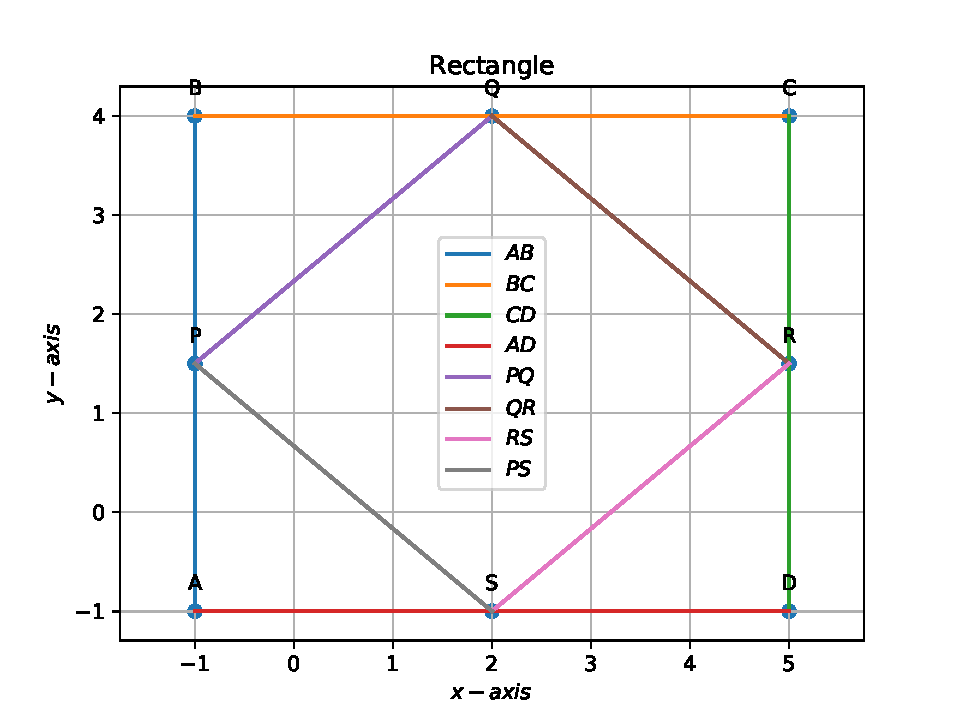
\includegraphics[width=\columnwidth]{./figs/problem1.pdf}
	\end{center}
\caption{}
\label{fig:Fig3}
\end{figure}
We know that PQRS is a parallelogram. To know, if it is a rectangle, we need to ascertain whether any of the two adjacent sides are perpendicular. 
That means $\brak{\vec{Q}-\vec{P}}^\top\brak{\vec{R}-\vec{Q}}$ should be equal to zero. \\
\begin{align}
\vec{Q}-\vec{P} &=  \myvec{
 2 \\
 4 \\
 } - \myvec{
 -1 \\
 \frac{3}{2} \\
 } = \myvec{
 3 \\
 \frac{5}{2} \\ 
 } \\
 \vec{R}-\vec{Q} &=  \myvec{
 5 \\
 \frac{3}{2}\\
 } - \myvec{
 2 \\
 4 \\
 } = \myvec{
 3 \\
 -\frac{5}{2} \\ 
 } \\ 
 \brak{\vec{Q}-\vec{P}}^\top\brak{\vec{R}-\vec{Q}} &= \myvec{
 3 & \frac{5}{2}} \myvec{
 3 \\
 -\frac{5}{2} \\
 } \neq 0
\end{align}
Therefore PQRS is not a rectangle. Let us check if it is a rhombus. For a rhombus, the diagonals bisect perpendicularly. That means $\brak{\vec{R}-\vec{P}}^\top\brak{\vec{S}-\vec{Q}}$ should be equal to zero. \\


\begin{align}
\vec{R}-\vec{P} &=  \myvec{
 5 \\
 \frac{3}{2} \\
 } - \myvec{
 -1 \\
 \frac{3}{2} \\
 } = \myvec{
 6 \\
 0 \\ 
 } \\
 \vec{S}-\vec{Q} &=  \myvec{
 2 \\
 -1 \\
 } - \myvec{
 2 \\
 4 \\
 } = \myvec{
 0 \\
 -5 \\ 
 } \\ 
 \brak{\vec{R}-\vec{P}}^\top\brak{\vec{S}-\vec{Q}} &= \myvec{
 6 & 0} \myvec{
 0 \\
 -5 \\
 } = 0
\end{align}
Therefore PQRS is a rhombus.

\end{enumerate}

\end{document}
